\documentclass{scu-thesis}

\usepackage{tabularx}
\usepackage{graphicx}
\usepackage{float}
\graphicspath{{images/}}

% \usepackage{graphicx}	% for including graphics
% \usepackage{amsmath}	% for advanced typesetting of mathematics
% \usepackage{txfonts}	% for using the Times-Roman font
% \usepackage{natbib}	% for better citation styles


% These must be set first ... the rest of the thesis commands rely on them.

\author{Maxwell Abrams}
\author{Cynthia Le}
\title{3D Bioprinter}
\department{Department of Computer Engineering}
\department{Department of Mechanical Engineering}
\department{Department of Bioengineering}
\degree{Bachelor of Science in Computer Science and Engineering}
\degree{Bachelor of Science in Mechanical Engineering}
\degree{Bachelor of Science in Bioengineering}


% Only bachelor's theses should have multiple authors and/or be from
% multiple departments.  Signatures required:
%
% Bachelor's theses: advisor(s), department chair(s)
% Master's theses: advisor, reader, department chair
% Doctoral theses: doctoral committee (including advisor), department chair

\begin{document}
\frontmatter
\signature{Thesis Advisor}
\signature{Thesis Advisor}
\signature{Department Chair}
\signature{Department Chair}

\maketitle
\begin{abstract}
A good abstract is a concise summary (1--2 paragraphs) of the entire
project: introduction, problem statement, work accomplished, results,
conclusions, and recommendations. When you write the abstract, imagine
that the reader will not read anything else, but that you must get
your major point across immediately. This requires efficiency of words
and phrases. An abstract is written to stand alone, without jargon or
reference to figures and tables in the report body.
\end{abstract}

Acknowledgments
\\
\\
Acknowledge the contributions of the sponsor, university staff, other students, faculty, and other persons who were of assistance. This section is optional.


\tableofcontents
\listoftables
\listoffigures

\mainmatter
\chapter{Introduction}

\section{Problem Statement}

 STEM (science, technology, engineering, and math) fields are a primary focus in education, because there is increasing need for students who have the technical skills to solve real-world problems. A major challenge that many STEM educators face is engaging students in the classroom. The education technology (ed-tech) startup, SE3D, hopes to solve this challenge by bringing 3D bioprinting technology to high school classrooms. Although SE3D has already produced a working prototype, the printer only has basic capabilities and requires further development.  

The 3D bioprinter senior design team aims to create a 3D bioprinter that can improve the capabilities of high school teachers to engage students in STEM education. Implementing 3D bioprinters into high schools will generate increased understanding and interest in biology, research, and technology for the students who will soon be America’s doctors, technicians, and scientific pioneers. 

In order to accomplish this goal, the team is expanding SE3D’s product line to improve student and teacher user experiences and to expand the possibilities for biological experiments. Table \ref{table:problem-solution} shows how SE3D’s current printer can be improved to meet these goals. 

\begin{table}[H]
\caption{\label{table:problem-solution} Current Bioprinter Problems and Senior Design Project Solutions}

\begin{tabularx}{\textwidth}{ |X|X| }
  \hline
  \textbf{Problem }& \textbf{Solution }\\

  \hline 
Printer lacks advanced features: automated camera, temperature control and humidity regulation

- Limits capability of experimentation

&  

Develop a separate, modular incubation unit (The Box) with an automated camera and humidity and temperature controls

- Analysis and printing can occur in parallel since functions are not in same physical space

- Automatic image capture to analyze experiment over time

- Simple user interface to configure and run experiments
 \\


    \hline 
 Printer only prints with one material

- Limits print designs
  & 
  Design and implement low cost dual extruder
   \\
  \hline
  Motion control system relies on specialized 3D printer software and feature-limited hardware

- Duet Control Board only supports basic 3D printing operations

- External computer necessary for control
&
Create custom software environment
- Distributed control board system to accommodate extra control features
Run on built-in computer 

- Keep low-cost with Raspberry Pi 

\\
  \hline
  Operator must manually calibrate syringe extruder

- Room for human error
&
Implement auto-calibration software of the syringe extruder
\\
  \hline
\end{tabularx}

\end{table}


The goals in Table \ref{table:problem-solution} are subject to the following criteria:
\begin{enumerate}
	\item Usable in a high school lab environment by both students and teachers
	\item Safe for all users
	\item Low cost
\end{enumerate}

% =======================================================================

% =======================================================================
\section{Background and Related Work}

The current bioprinter produced by SE3D, the r3bEL, is marketed towards high school science classes. It prints using a single 5 mL syringe that has to be manually loaded by the user, put into the head of the bioprinter, and calibrated by hand to begin printing. It currently has the capability to print enzyme, alga, and bacterium 2D arrays, chocolate, and cells and scaffolds for 3D tissue engineering. The r3bEL printer can print four 3x3 array tray experiments in about 3 minutes. After it is finished, the experiment must remain on the bed of the bioprinter until it finishes culturing. The user gathers data form the experiment by constantly taking pictures of the experiment as it cultures. To capture more consistent and higher quality images, an SE3D employee created a separate box that block out external light and has its own light source. This small box has a removable ceiling, lined with LEDs, and holds a single Petri dish. A small hole in the ceiling allows a mobile phone camera to be placed over it to capture images of the experiment as it cultures, though it still requires an individual to operate the camera and capture each image.


\begin{table}[H]
\caption{\label{table:printer-comparison} Comparison of Existing 3D Bioprinters}
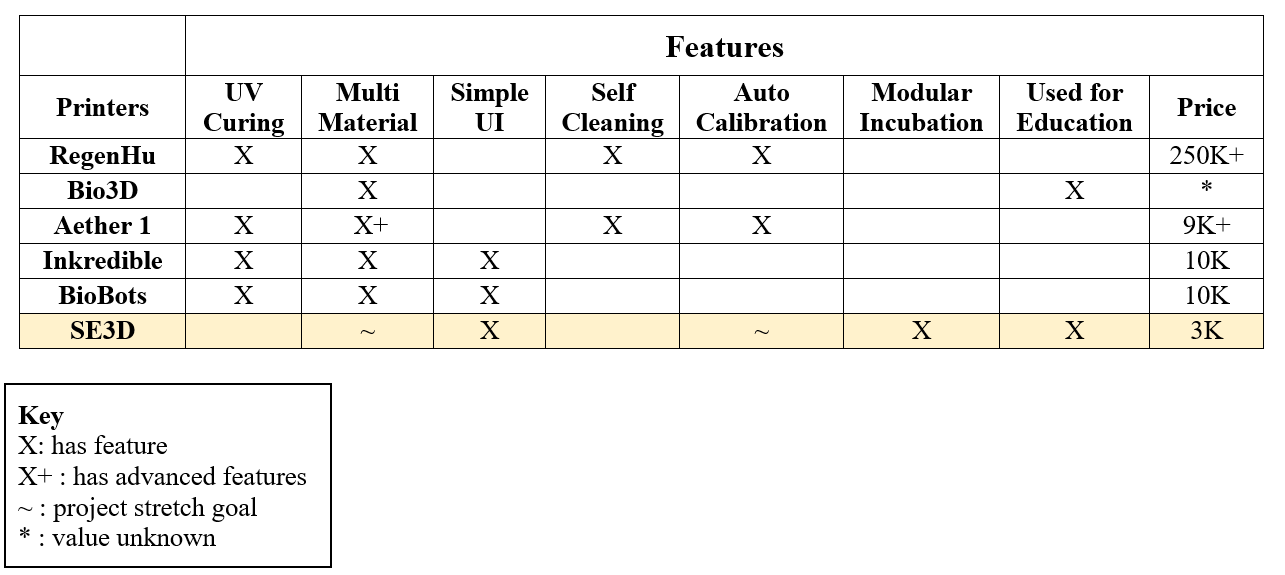
\includegraphics{printer-comparison-table}
\end{table}
Although the team is enhancing the functionality of SE3D’s 3D Bioprinter, there are currently many similar products that are already available for purchase. Below are the bioprinters shown in Table \ref{table:printer-comparison} with an explanation of their key features and price ranges.



\textit{RegenHu: 3D Discovery Printer} \\
RegenHu produces a professional printer priced at 250,000+ USD. It supports a wide range of funcationalities and applications. It is primarily used for optimal processing of a broad biomaterial/bioactives portfolio. The device prints using cell-friendly Ink-jet and thermopolymer extrusion using a 2-component printhead. In addition, it has a high precision temperature controller for biomaterial culturing.

\textit{Bio3D Technologies: Bio3D Explorer Series}\\
Three-dimensional bioprinters have also been developed internationally. Bio3D Technologies in Singapore has a series of printers in their Explorer product line. Designed for educational purposes, the Bio3D has 1 to 4 printing heads available and is lightweight and foldable with a full metal frame. The device is suitable for a wide range of applications and materials. The price was not listed online.

\textit{Aether 1 3D Bioprinter} \\
Aether has a 3D bioprinter that begins with a base unit cost of 9,000 USD. The product includes 8 syringes, 2 hot ends, and 10 extruder print heads. It has the widest range of usable materials for printing, from oils to plastics. The device has many useful attachments, like a UV curing light for biomaterial prints. Its extruders are pneumatic-driven.

\textit{CellInk: Inkredible Printer} \\
In Palo Alto, California, CellInk manufactures a research grade bioprinter, Inkredible. Inkredible is priced at 10,000 USD for the base version of the printer. It focuses on assisting tissue engineers who use their custom bioink line to create hydrogel structures that allow for efficient mammalian cell culturing. It has been optimized to print skin and cartilage tissue and uses UV lighting to cure the biomaterial. The printer has a clean chamber and heated cartridges.

\textit{BioBots 3D Printer} \\
BioBots has a desktop 3D printer capable of printing tissues out of living cells. The base model price of BioBots’ 3D printer is 10,000 USD. It is small and portable to allow for ease of use. In addition, the device has a dual heated, pneumatic driven extruder system for precise printing and uses replaceable syringes for easy material changing. Blue light technology is used to safely cure the biomaterial. BioBots is based in Philadelphia; however, they ship internationally.

After reviewing these printers, it is clear that they are all capable of completing the biological experiments that SE3D desires. The one aspect that they all do not meet, however, is that they are priced much higher than the average high school laboratory budget. Furthermore, these printers require high levels of knowledge in order to operate, which is not a reasonable expectation of high school students. To improve this aspect, the UI must be simplified and easy to use for people with less than a high school education. The closest competitors are Inkredible and BioBots, which are low cost and have simple user interfaces. The 3D Bioprinter that the team is working on improves on this problem by providing the necessary functionality at a more reasonable price closer to 3,000 USD. 


% =======================================================================

% =======================================================================

\section{Objectives}

The 3D bioprinting team consists of mechanical engineers, computer engineers, and bioengineers. To accomplish the project goals, the team has split the project into three parts: The Box, 3D Printing Feasibility Study, and a bioengineering experiment. The bulk of this document will focus on the software components for The Box and 3d Printing feasibility study, as that will be where the computer engineering work is applied.
\begin{itemize}
	\item  The Box:
	\begin{enumerate}
		\item Meet with Maya, SE3D CEO to define requirements for the incubating box
		\item Make design decisions for functionality included in the box and physical and structural designs
		\item Develop prototypes of box, user interface, and controls, allowing users to customize the box environment, begin and end experiments, and automatically capture a series of photos
		\item At every stage of development, run tests for proper software and hardware compatibility
		\item Share prototype with users in a classroom setting for feedback
	\end{enumerate}
	\\
	\item 3D Printer Feasability Study:
	\begin{enumerate}
		\item Analyze usability of the SE3D bioprinter and identify areas of improvement.

		\item Incorporate an auto-calibration mechanism for the syringe plunger though physical designs and adaptation of printer firmware.

		\item Extend printer functionality to two extruders for multi-material extrusion of biomaterial and the other PLA.

		\item At every stage of development, run tests for proper software and hardware compatibility.

		\item Share prototypes with stakeholders for feedback.
	\end{enumerate}
\end{itemize}
\chapter{Requirements}

The requirements section defines and qualifies what our 3D printer feasability study and the incubating box must do. We communicated with SE3D to determine the requirements.

\section{Functional Requirements}

Functional requirements define what the system must do. \\
The incubating box system will:
\begin{itemize}
	\item support timed image capture at a pre-specified image per time interval
	\item have an interactive user interface
	\item allow user to monitor and control light, temperature, and camera settings
	\item allow users to download captured images
	\item allow users to save settings as custom environments to be used later
\end{itemize}


The 3D printer feasability study system will:
\begin{itemize}
	\item show feasability of auto-homing of SE3D's syringe 
	\item show feasability of adding a multi-material printing module to an open source printer
\end{itemize}

% =======================================================================

% =======================================================================

\section{Non-Functional Requirements}
Non-functional requirements define the manner in which the functional requirements need to be achieved. \\
The system will be:
\begin{itemize}
	\item User friendly and intuitive
	\item Safe
	\item Secure
	\item Reliable
\end{itemize} 
% =======================================================================

% =======================================================================

\section{Design Constraints}
Design Constraints are non-functional requirements that constrain the solution instead of the problem. \\
The system must:
\begin{itemize}
	\item function without being connected to a desktop or laptop computer
	\item be low- cost
\end{itemize}


\chapter{Use Cases}

Use Case diagrams define tasks that users will perform to achieve a certain goal when using our incubating box and 3d bioprinter system.

\section{The Box}

\begin{figure}[H]
\caption{\label{figure:box-use-case} Use Case Diagram for The Box}
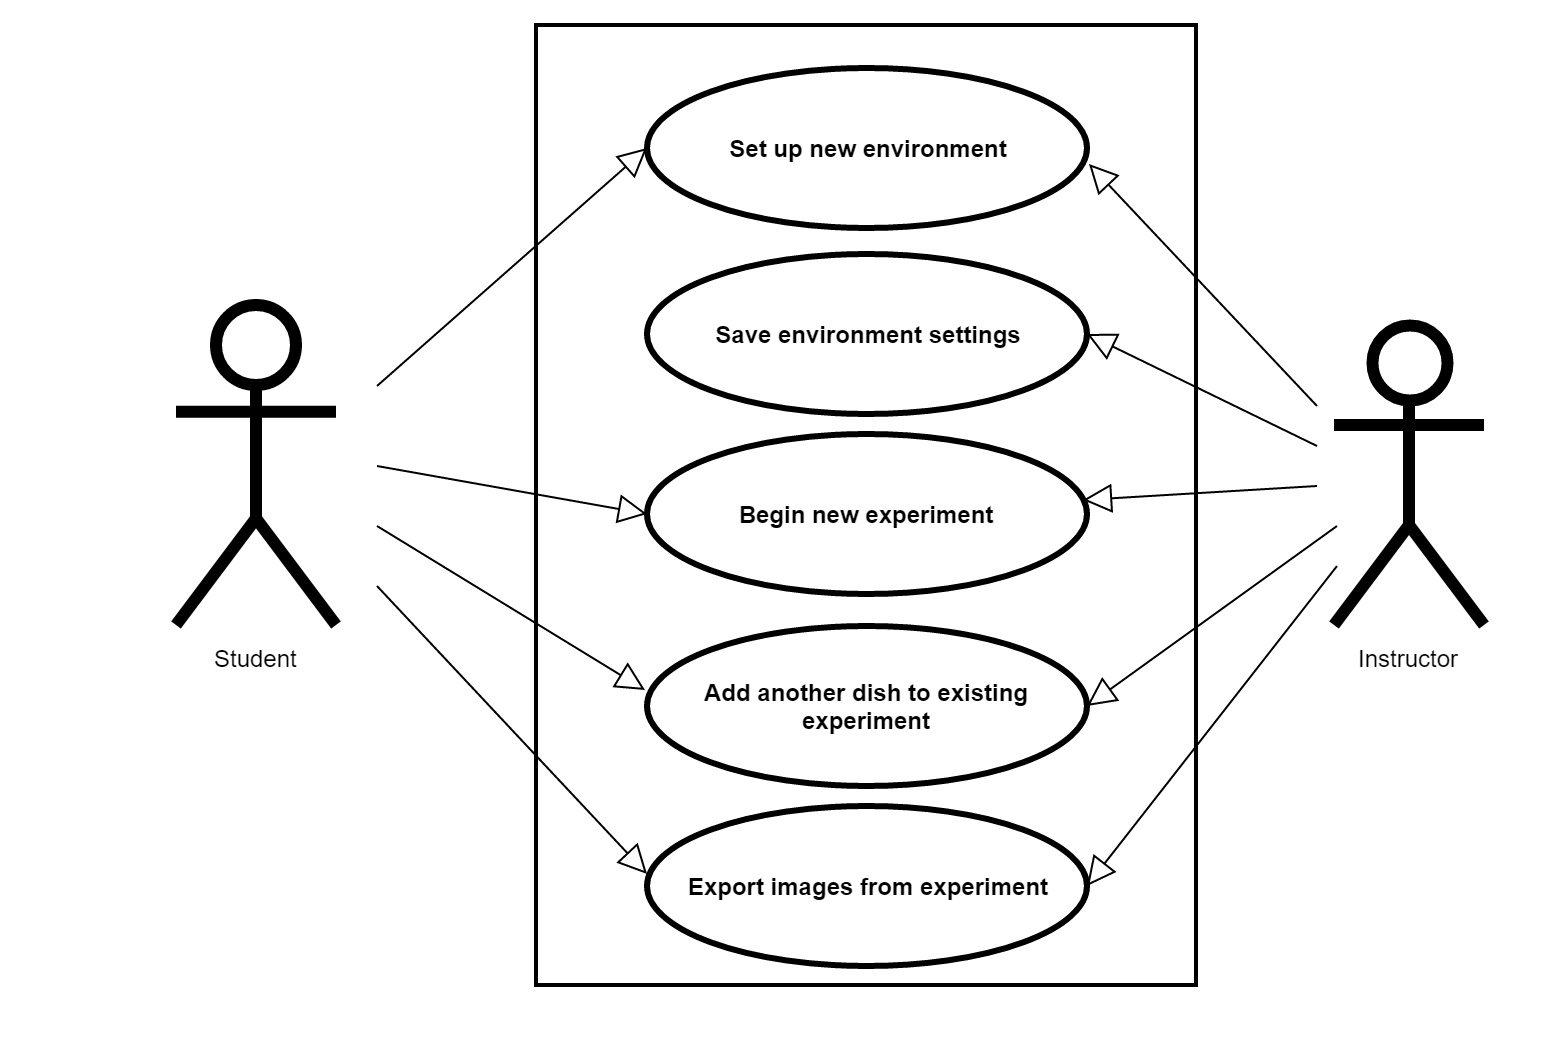
\includegraphics{box-use-case}
\end{figure}

\begin{enumerate}
	\item 
	\begin{itemize}
		\item Name: Set up new environment
		\item Goal: Prepare The Box to have the proper settings for the experiment that the user wants to run
		\item Actors: Student, Instructor
		\item Pre-conditions: No other experiment is currently running
		\item Steps: Either load settings that have been previously saved, or enter custom light, temperature, and image capture settings. 
		\item Post-conditions: The Box is at currect environment settings for the experiment.
		\item Exceptions
	\end{itemize}
	\item 
	\begin{itemize}
		\item Name: Save environment settings
		\item Goal: Save temperature, light, and image capture settings to prevent repetition in the future
		\item Actors: Student, Instructor
		\item Pre-conditions: User has input custom temperature, light, and image capture settings
		\item Steps: User clicks `Save Custom environment' and enters an appropriate name
		\item Post-conditions: Future users will now be able to load this environment for future experiments
		\item Exceptions: n/a
	\end{itemize}
	\item 
	\begin{itemize}
		\item Name: Begin new experiment
		\item Goal: Begin timer and image capture on current incubated experiment
		\item Actors:  Student, Instructor
		\item Pre-conditions: User has entered proper environment settings, selected which petri dishes are present, and has placed petri dishes in The Box. The Box has been brought to proper temperature.
		\item Steps: Click `Begin Experiment'
		\item Post-conditions: Timer and image capture begins
		\item Exceptions: n/a
	\end{itemize}
	\item 
	\begin{itemize}
		\item Name: Add another dish to existing experiment
		\item Goal: Add another dish to a experiment that is already running 
		\item Actors:  Student, Instructor
		\item Pre-conditions: An experiment must be running in The Box
		\item Steps: User places dish in the box. Clicks on the appropriate petri dish to begin timer and image capture of new dish
		\item Post-conditions: New petri dish is added into the experiment and final end time is extended to accommodate 
		\item Exceptions
	\end{itemize}
	\item 
	\begin{itemize}
		\item Name: Export images from experiment
		\item Goal: Download images captured during the experiment of a single petri dish for analysis
		\item Actors:  Student, Instructor
		\item Pre-conditions: A USB drive has been inserted and detected
		\item Steps: Click `download images' button, Select the relevant dish, click `download'
		\item Post-conditions: Images transferred onto the USB drive
		\item Exceptions
	\end{itemize}
\end{enumerate}
\section{Feasability Study}
\chapter{System Sequence Diagrams}

\section{The Box}
\section{Feasability Study}
\begin{figure}[H]
\includegraphics[scale=0.5]{3D_Printer_Activity_Diagram1}
\caption{\label{figure:3D_Printer_Activity_Diagram1} Activity digram for user starting a print on the 3D printer}
\end{figure}

\begin{figure}[H]
\includegraphics[scale=0.5]{3D_Printer_Activity_Diagram2}
\caption{\label{figure:3D_Printer_Activity_Diagram2} Activity digram for user stopping a print on the 3D printer}
\end{figure}
\chapter{System Design- The Box}

The Box is a stand alone, modular incubator that will be used to let certain SE3D experiments culture over an extended period of time. It will provide a custom lighting environment that allows consistent lighting conditions for the camera to effectively document the experiments. The box also will have temperature control capabilities to adjust temperature levels for each of the relevant SE3D experiments. The box will support nine petri dishes at one time.

\begin{figure}[H]
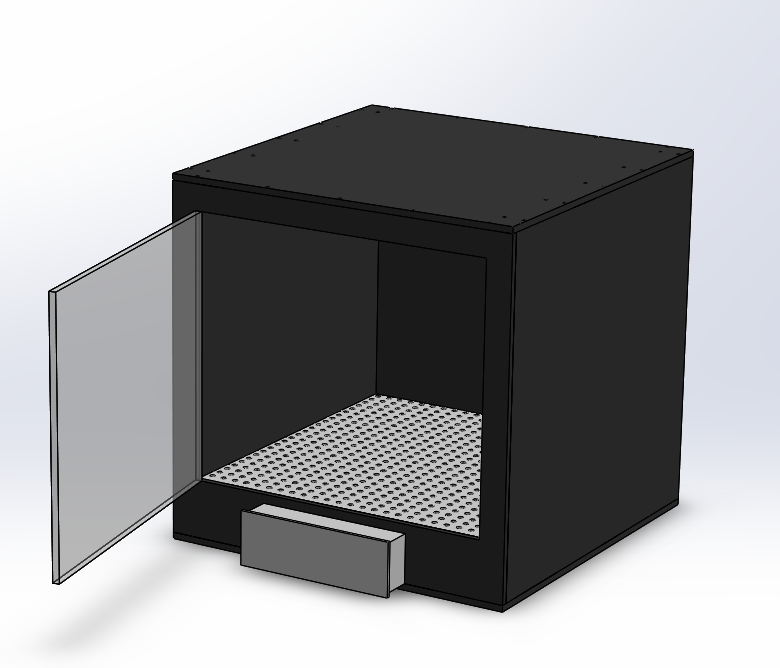
\includegraphics[scale=0.5]{box}
\caption{\label{figure:box} Initial Incubator Prototype}
\end{figure}

Figure \ref{figure:box} shows a initial drawing of the plans for the physical incubating box. At the top of the box, there will be a touch screen that allows users to interact with the controls of The Box.

% =======================================================================

% =======================================================================

\section{Architectural Design}


\begin{figure}[H]
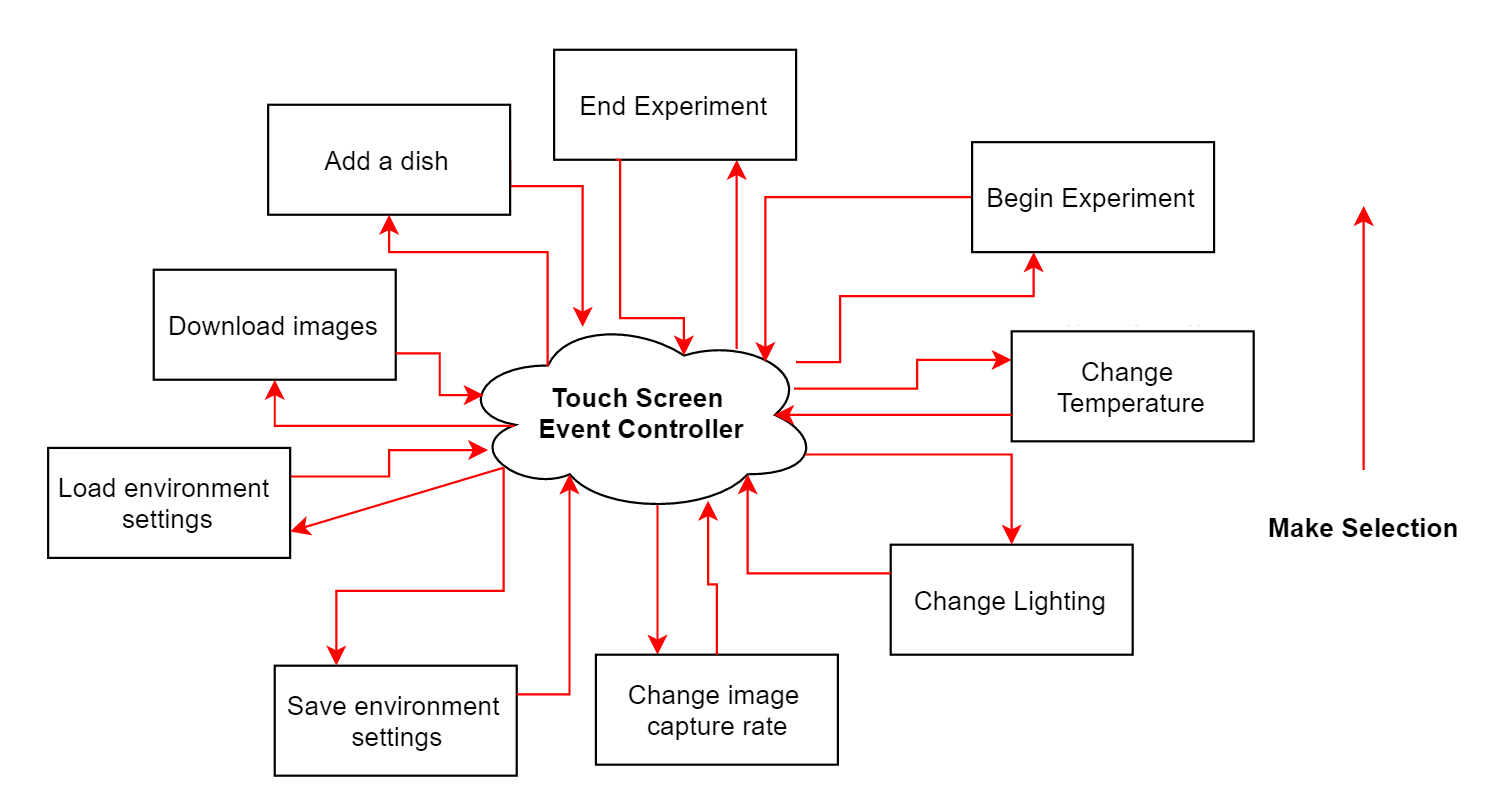
\includegraphics[scale=.8]{box-arch-diagram}
\caption{\label{figure:box-arch} Architectural design of event based incubator box system}
\end{figure}

The Box will  study will operate on an event based architecture. The user can interact with the system and move between system states by selecting options on the touch screen.


% =======================================================================

% =======================================================================
\section{Conceptual Model}

The user interface for The Box consists of screens in which the user can configure the box’s settings for the current experiment, begin and end experiments, and download images that are collected during the experiment. The user interface shall perform the following: 

\begin{enumerate}
	\item	Run off of a microcomputer
	\item	Allow users to choose custom light, temperature, and image capture settings
	\item   Allow users to save a set of environment settings
	\item	Allow users to load a previously saved environment 
	\item	Organize all images from a single experiment into a folder per petri dish so that they each can be exported to USB 

\end{enumerate}

\begin{figure}[H]
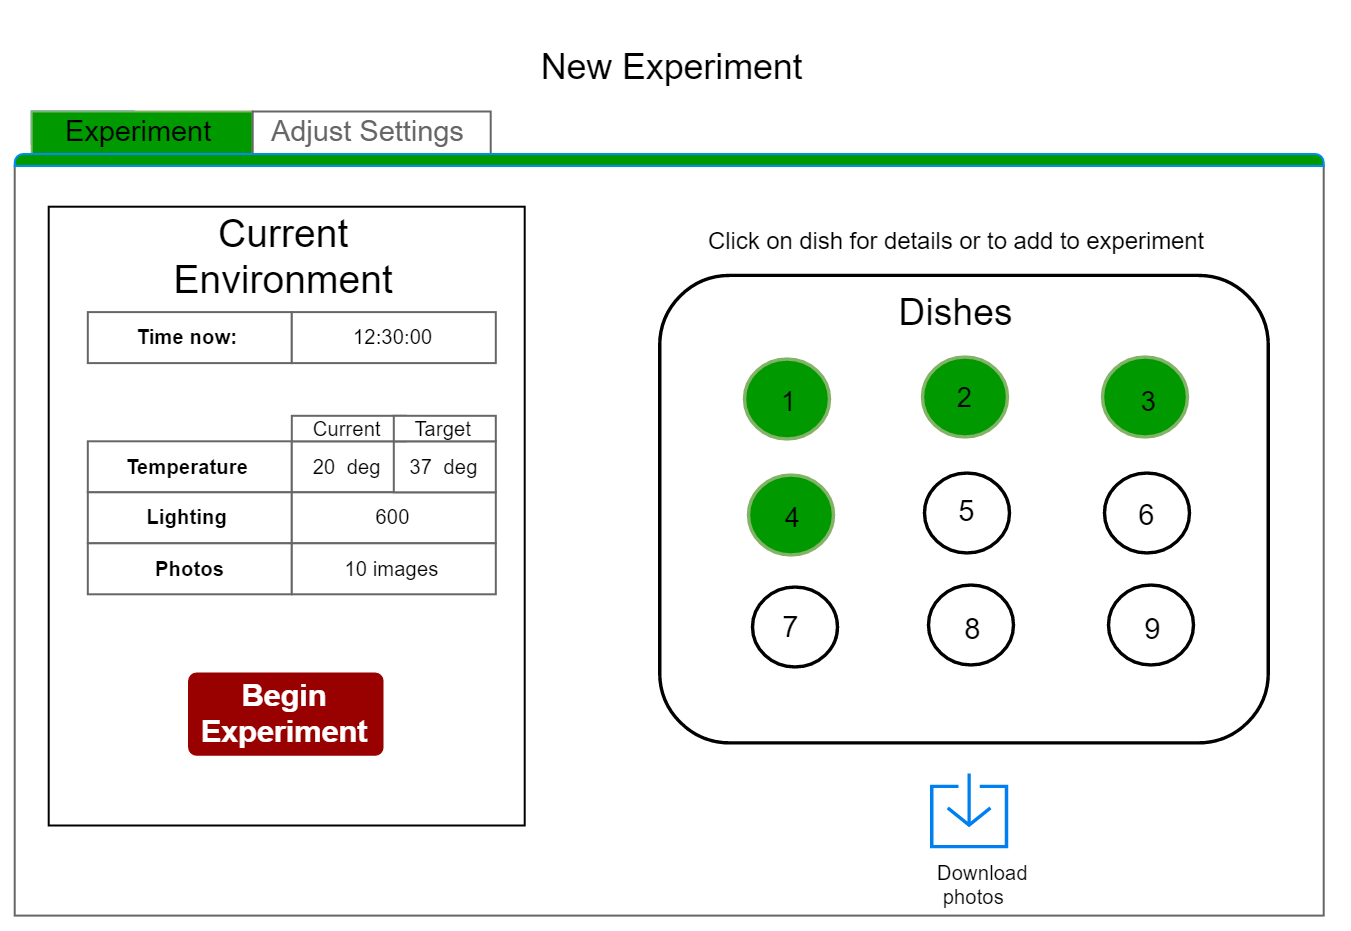
\includegraphics[scale=0.5]{ui-home-screen}
\caption{\label{figure:ui-home} Mock up of home screen}
\end{figure}

The user interface mock-ups shown in Figures \ref{figure:ui-home} through \ref{figure:ui-image} step through a typical sequence of steps a user would take when using the sytem. The first screen show, in Figure \ref{figure:ui-home}, is the default home screen that is shown when a experiment is not running. The home screen shows current environment status of the box. If a user would like to begin a new experiment, he would first select the dishes that will be initially placed into the incubator by clicking on each numbered circle that corresponds to a specific location inside of the physical box. Figure \ref{figure:ui-home} shows dishes 1-4 will be present in the experiment. 

\begin{figure}[H]
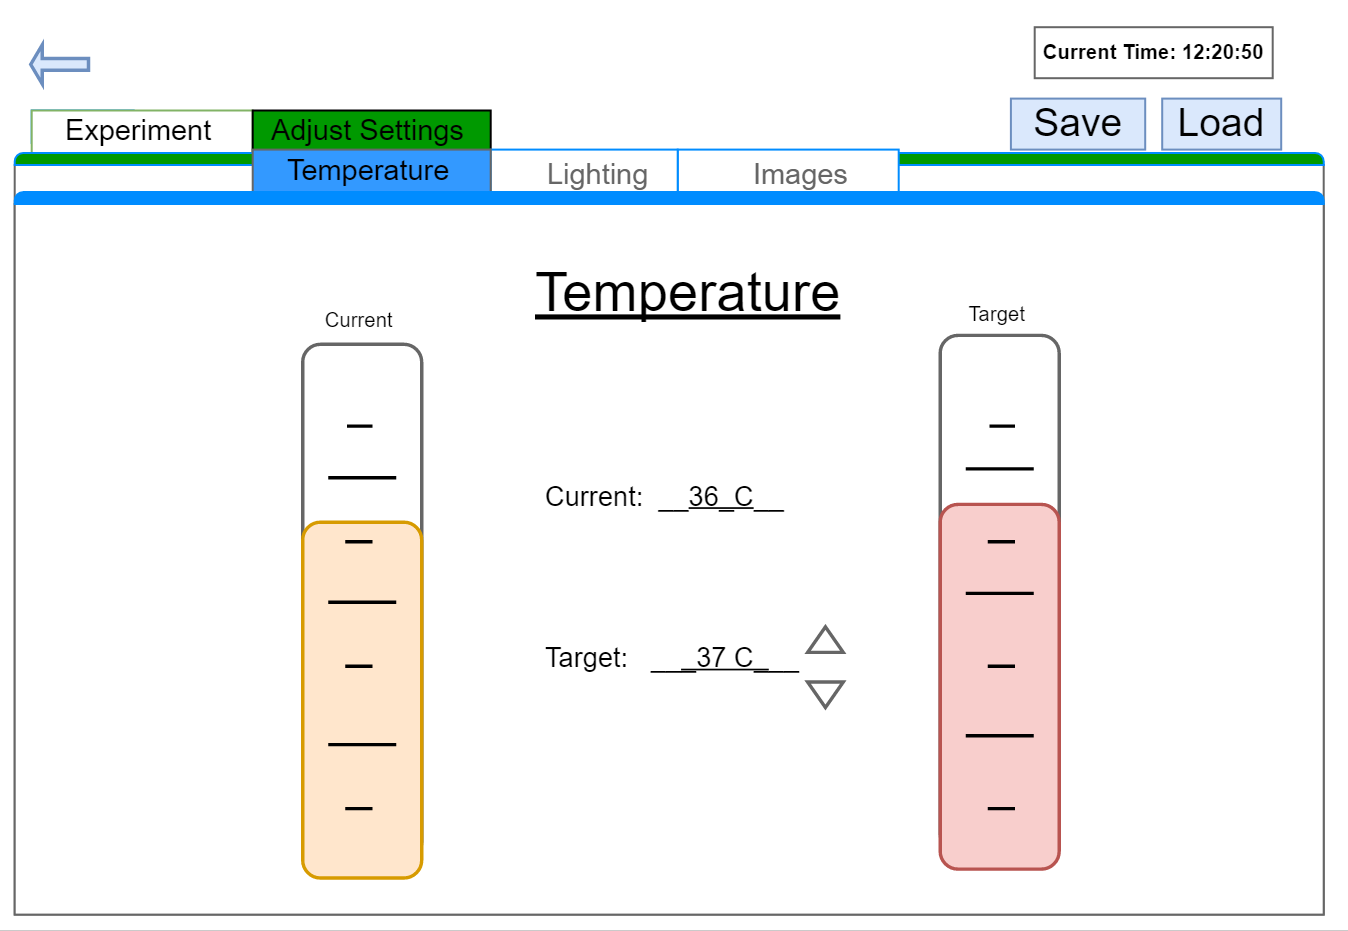
\includegraphics[scale=0.5]{ui-temp}
\caption{\label{figure:ui-temp} Mock up of temperature setting}

\end{figure}

\begin{figure}[H]
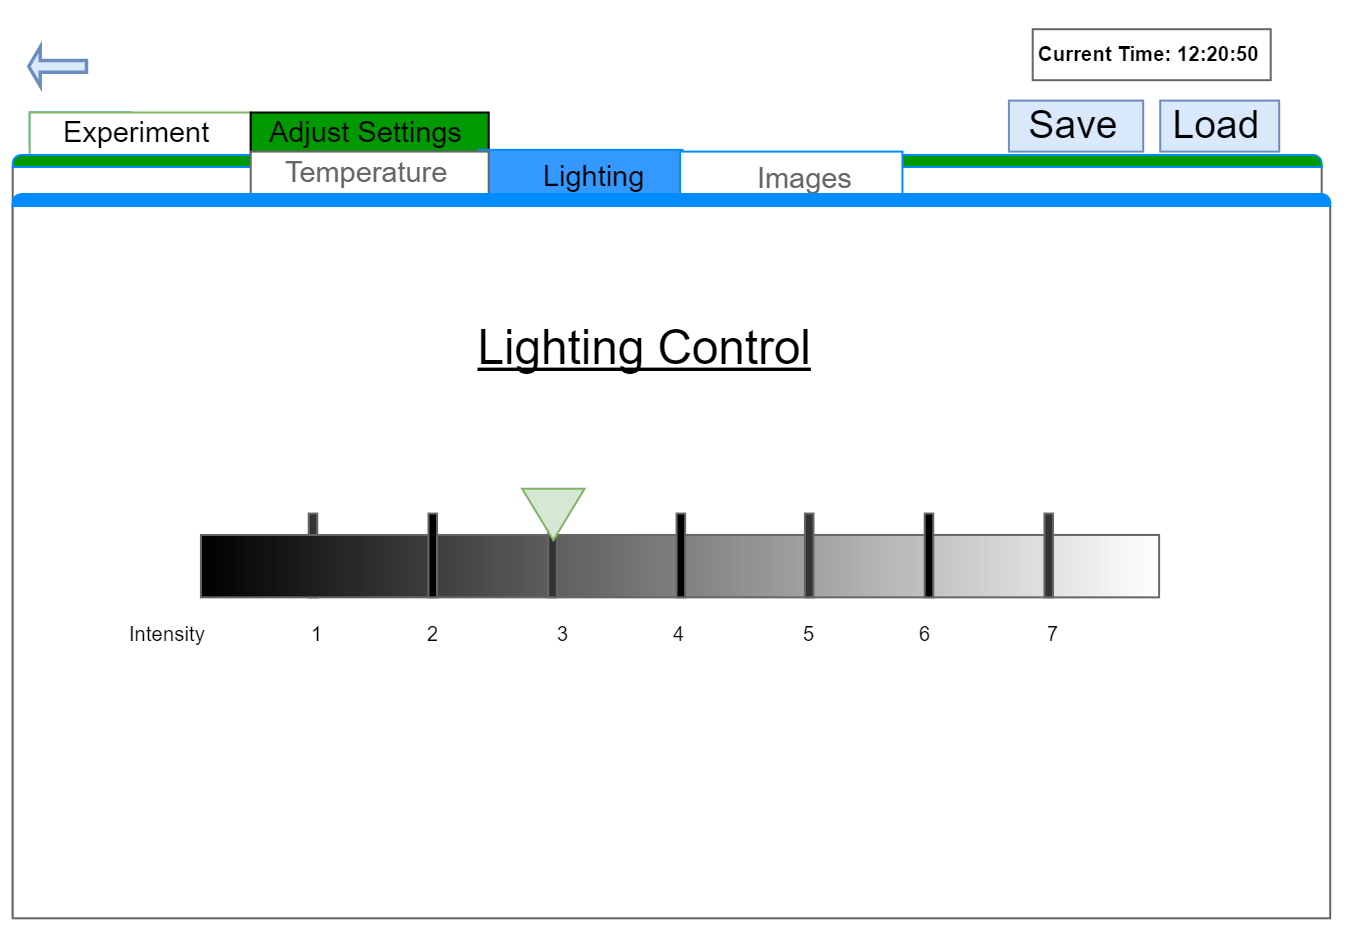
\includegraphics[scale=0.5]{ui-light}
\caption{\label{figure:ui-light} Mock up of light intensity setting}
\end{figure}

\begin{figure}[H]
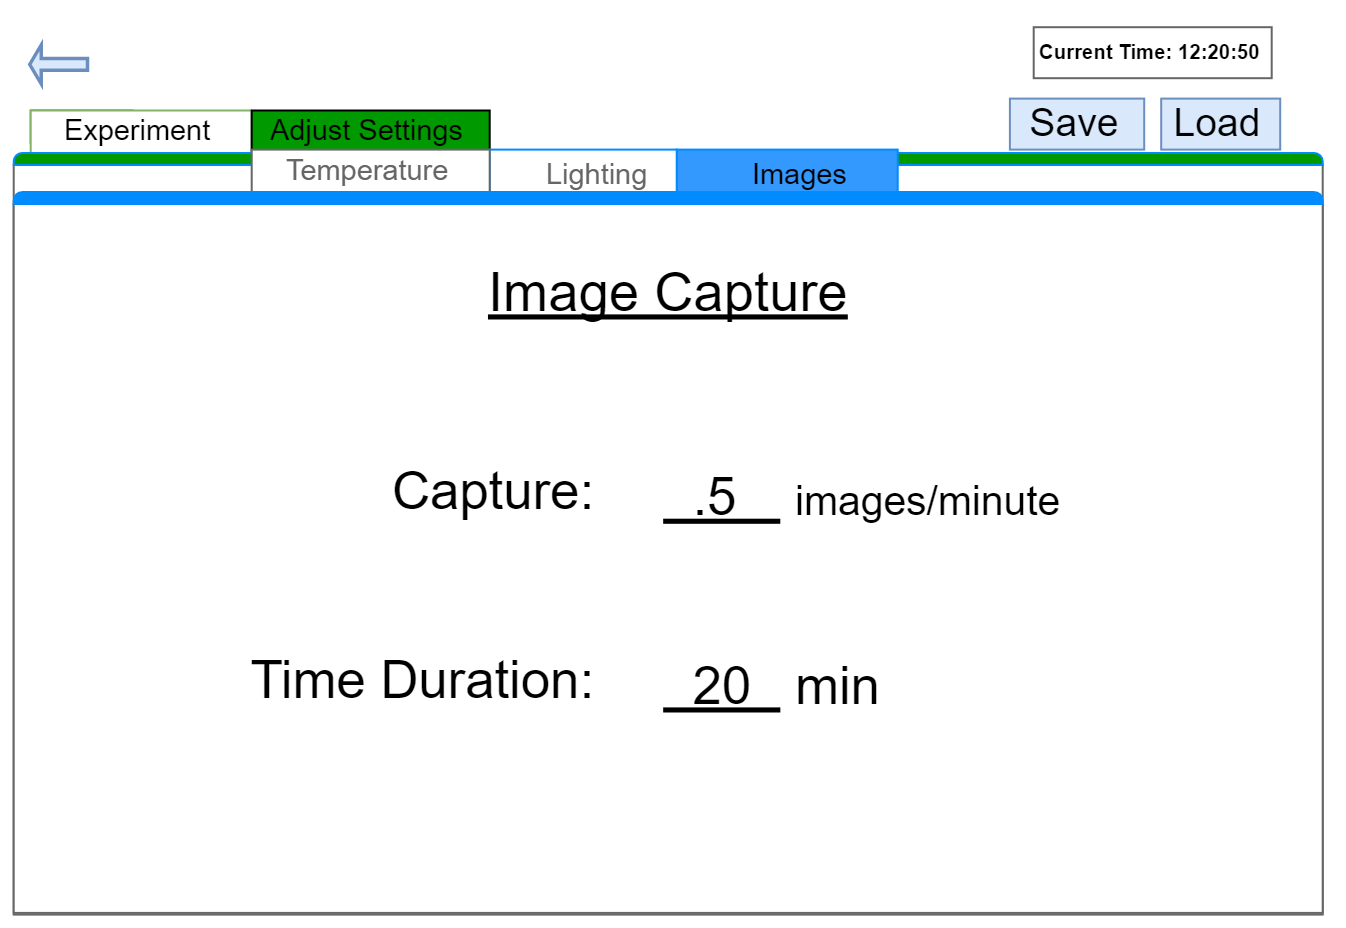
\includegraphics[scale=0.5]{ui-image}
\caption{\label{figure:ui-image} Mock up of image capture setting}
\end{figure}


Next, to customize the environment, the user would click adjust settings to be taken to the settings panel, shown in Figures \ref{figure:ui-temp} through \ref{figure:ui-image}. The user can choose to load a previously saved set of environment settings or provide a new set of environment settings. In each of these panels, the user can choose the appropriate temperature, light, and image capture settings for the system. After, he can choose to save the set of settings to be used in the future. 

\begin{figure}[H]
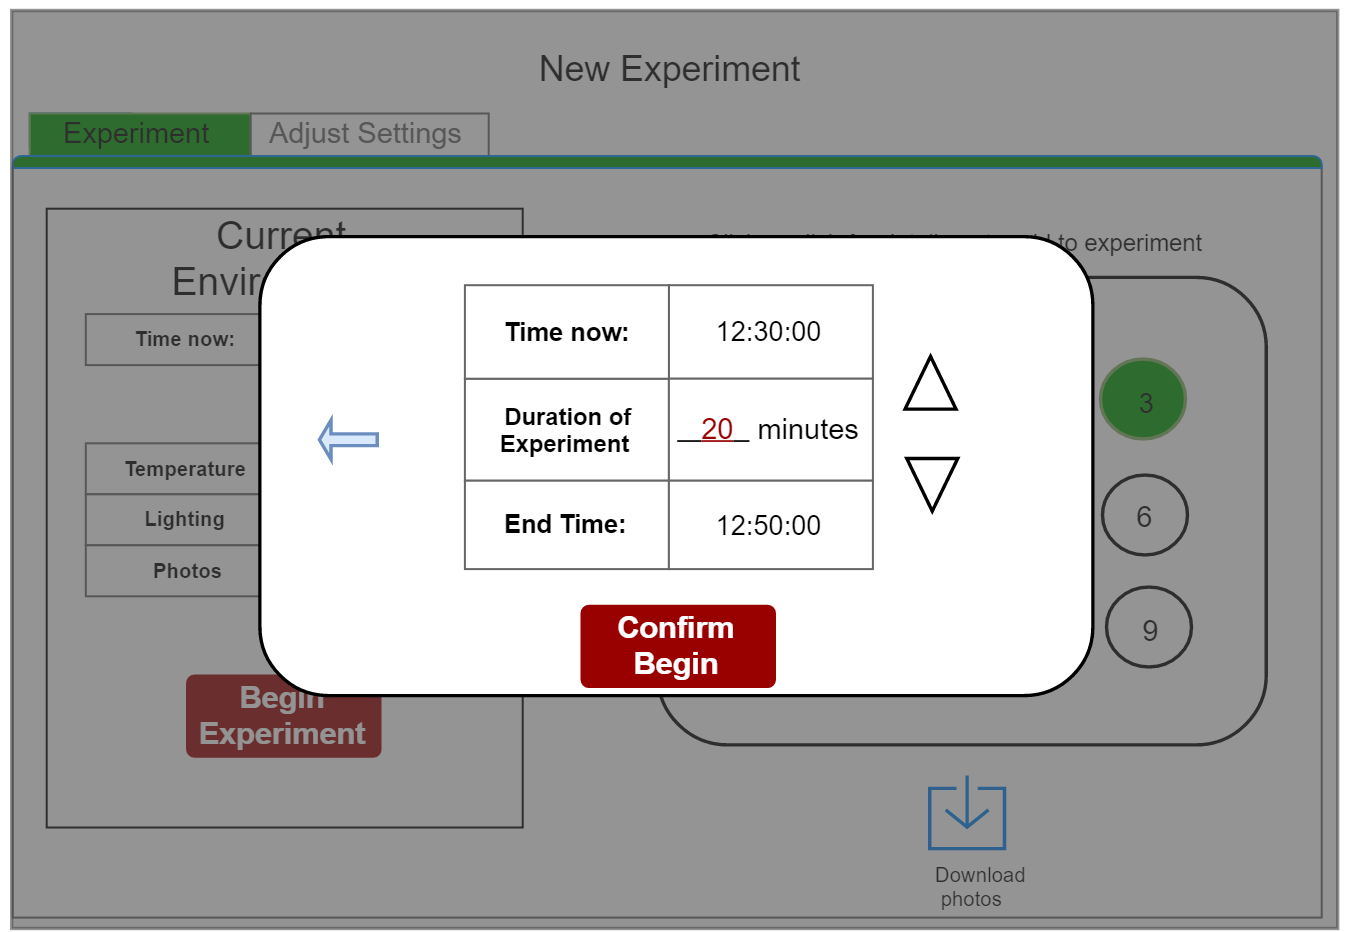
\includegraphics[scale=0.5]{ui-begin}
\caption{\label{figure:ui-begin} Mock up confirming experiment begin }
\end{figure}


Once the settings are appropriately chosen, the user navigates back to the home page to begin the experiment. The user clicks the `Begin Experiment' button and a confirmation screen will pop up to allow users to specify how long the incubating box will maintain the environment. This is shown in Figure \ref{figure:ui-begin}.


\begin{figure}[H]
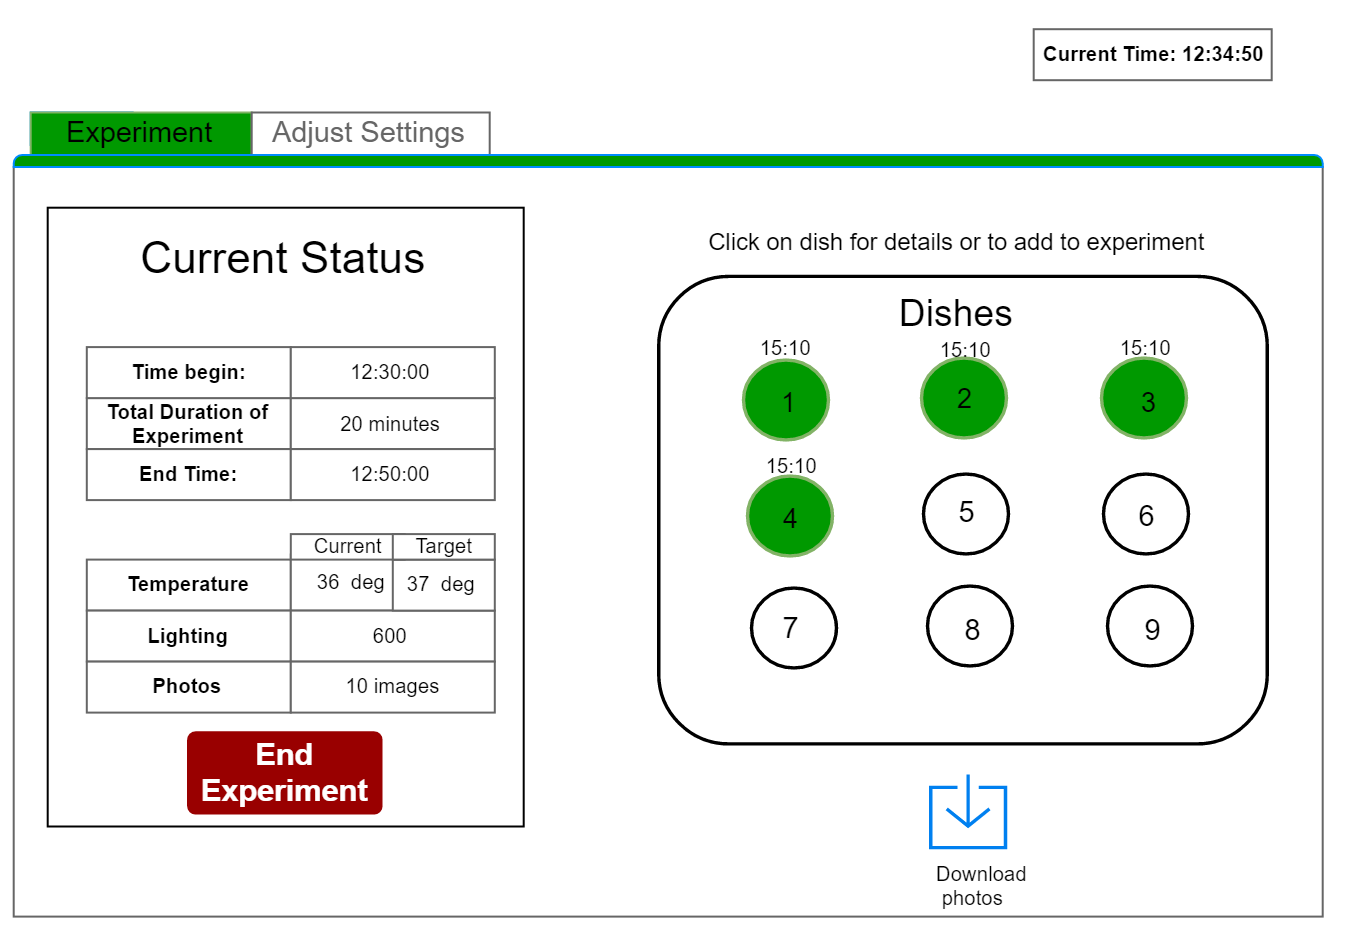
\includegraphics[scale=0.5]{ui-status-1}
\caption{\label{figure:ui-status} Mock up of status screen during an experiment}
\end{figure}

\begin{figure}[H]
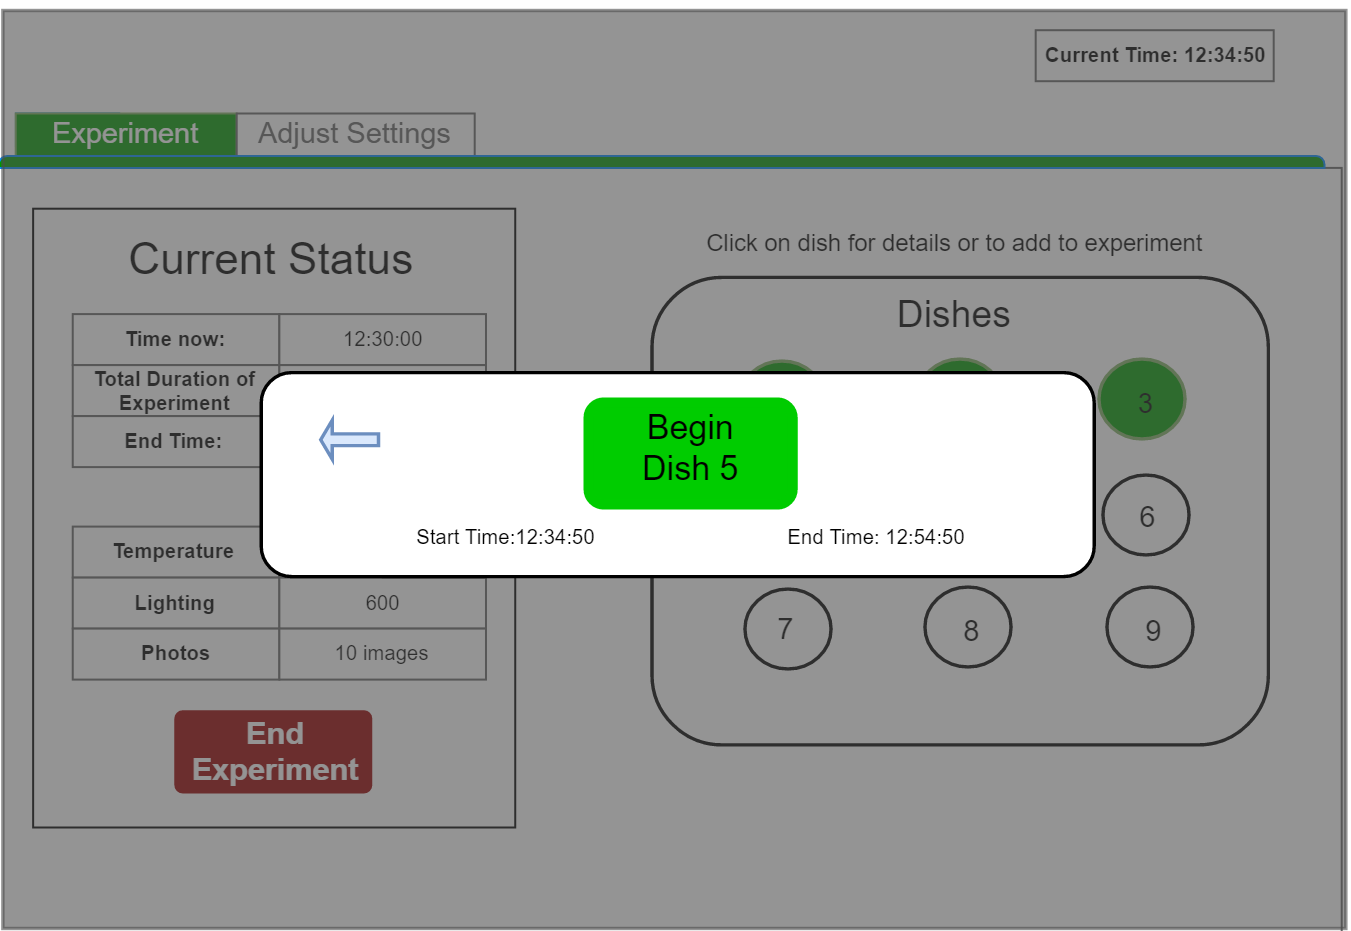
\includegraphics[scale=0.5]{ui-add-dish}
\caption{\label{figure:ui-add} Mock up of how a dish is added in the middle of an experiment}
\end{figure}

\begin{figure}[H]
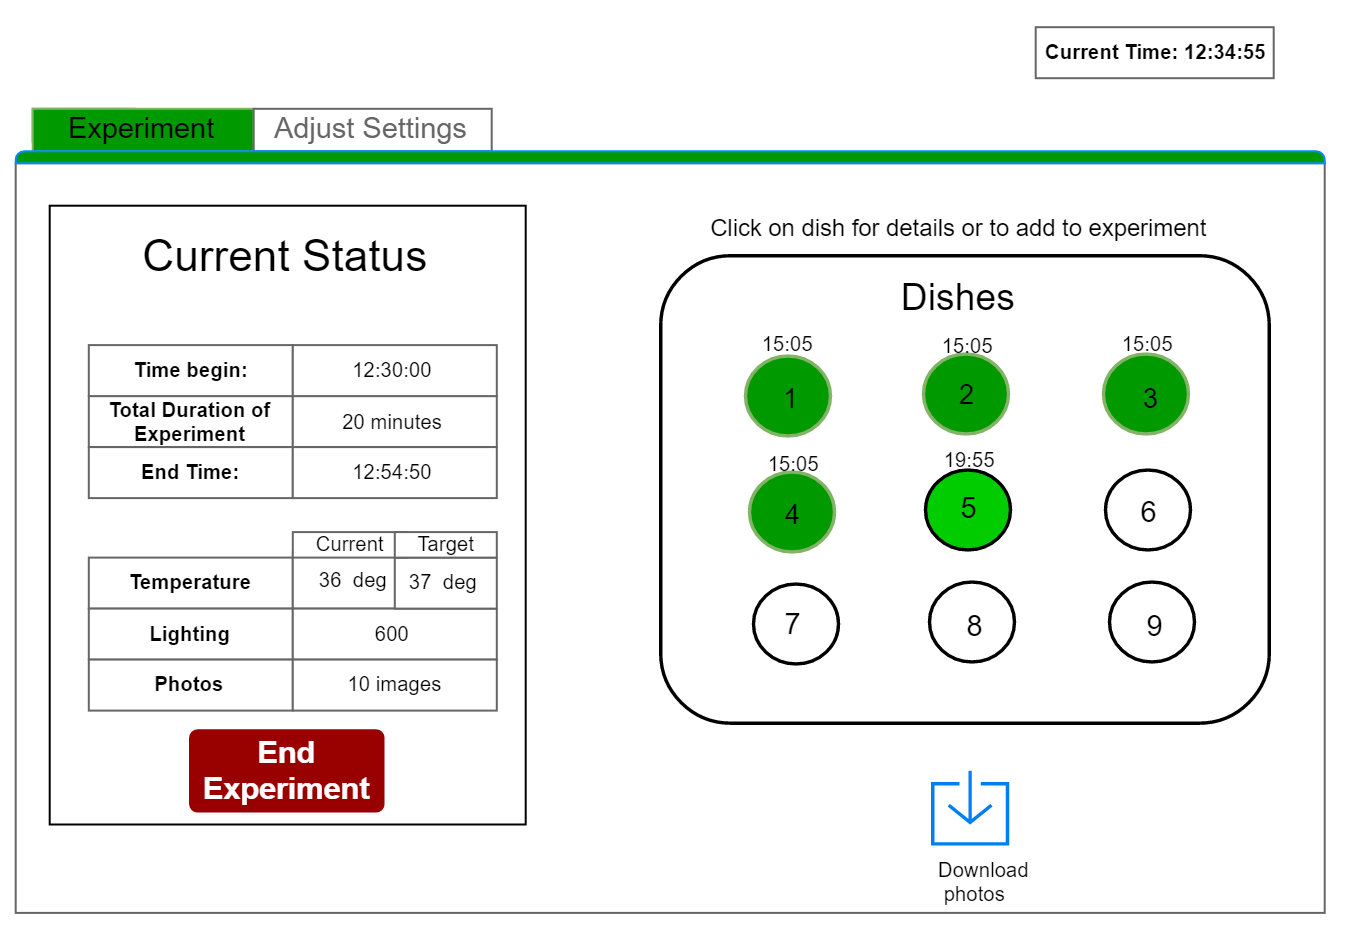
\includegraphics[scale=0.5]{ui-after-add}
\caption{\label{figure:ui-after-add} Mock up of how current status screen reflects addition of a dish}
\end{figure}

As seen in Figure \ref{figure:ui-status}, users will be able to monitor the experiment in real time and see how much time is left in the experiment as well as the current incubator conditions. If another dish needs to be added into the incubator in the middle of a running experiment, the user will add the dish into the box, then click on the corresponding circle on the screen. Figure \ref{figure:ui-add} shows Dish 5 being added into the experiment.  After the dish is added, the current staus screen is updated appropriately to reflect the change- specifically in the duration of experiment and end time sections as well as in the `Dishes' graphic. This is show in Figure \ref{figure:ui-after-add}.


\begin{figure}[H]
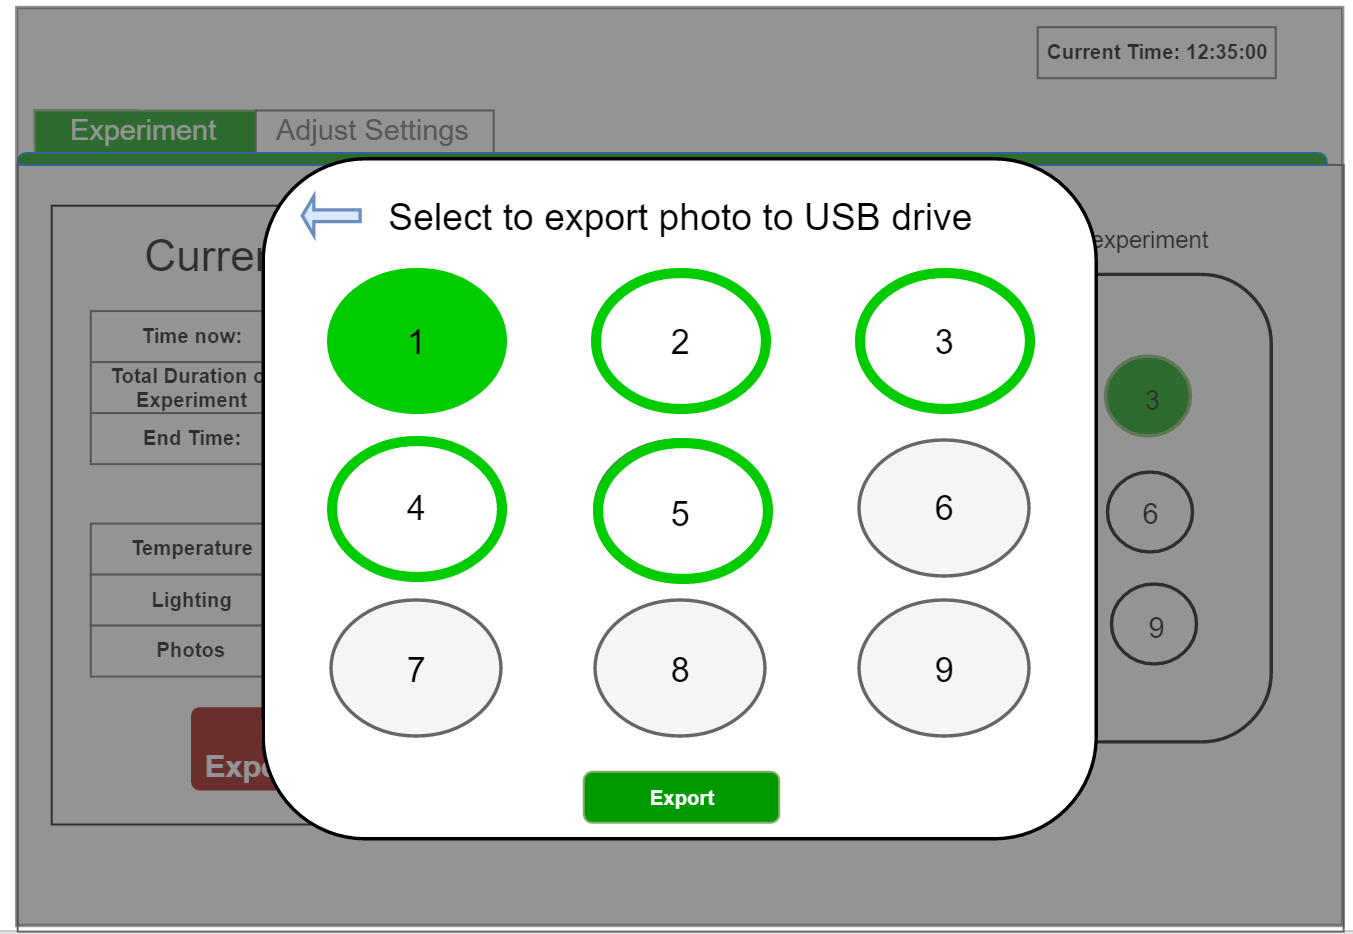
\includegraphics[scale=0.5]{ui-export}
\caption{\label{figure:ui-export} Mock up of export images to a USB drive}
\end{figure}

After an experiment is finished, users will export the images captured by USB. After a USB drive is inserted and recognized by the system, the user can click `Download Photos' on the status screen. A pop-up will allow the user to choose which dish's images the user would like to export. In Figure \ref{figure:ui-export}, the images of Dish 1 will be exported to the USB drive.



% =======================================================================

% =======================================================================
\section{Technologies Used}
	\begin{itemize}
	\item Git: A commonly used version control system. Git allows distributed workflow with high data integrity.
	\item Raspberry PI: A small, commonly used open-source computer with large community support. The Raspberry PI has General Purpose Input/Output (GPIO) pins for interfacing with other devices as well as built in WIFI, Bluetooth, GPU with HDMI output, and USB support.
	\item Java - A class based, object oriented computer programming language that is used for general purpose computing. Java is commonly found in projects around the world.
	\end{itemize}

% =======================================================================

% =======================================================================
\section{Design Rationale}
\subsection{Justification of User Experience}

We decided a touch screen interface was the most effective solution for the most enjoyable user experience for both high school students and instructors. A touch screen interface provides better image quality and intuitive interaction for users. Users are familiar with touch screens because of the popularity of touch screen smart phones and other screens.

The user interface is optimized for a touch screen experience. Since users will be using fingertips to navigate the interface, instead of a mouse cursor or stylus, all functions are tied to simple and prominent buttons. We kept the interface as simple as possible, only showing options and information that are necessary. Since we anticipate that we will have about a 5 in. screen, a simpler interface allows users to more easily navigate the system. In addition, since our users will be high school students, limiting the options they have on each screen reduces confusion on what to do next and lowers the chance of error due to unintentional clicks of other buttons.

There is minimal direct user input of values to reduce the need for on-screen keyboards that can be hard to navigate on a small screen. Instead, numbers are increased or decreased with up and down arrows, images, text, and color highlighting are used for signaling if certain dishes are selected or in use, and sliders are used in configuration. Reducing direct user input reduces  the likelihood of human error.

We chose not to include preloaded experiment settings that users can choose from after speaking with Maya from SE3D. Allowing users to input their own settings provides more flexibility for the user to customize experiments and create their own experiments. Since there are only a few criteria to set- light, temperature, image capture, and duration of experiment- it does not add too much overhead in set-up time. Users will have the option to save a certain combination of environment settings to use in the future. Thus, the `preloaded experiment' feature is emulated here- an instructor could set up a desired environment before class begins and save it to the system. Students can then load the environment that was set up by their instructor. 


\subsection{Justification of Technologies Used}
\begin{itemize}
	\item Git: Git was chosen because of its ability to store nearly any type of electronic materials such as images, source code, and documentation. It is commonly used in industry and is well supported. It allows the developers to work concurrently on various parts of the project which results in much faster completion times. Finally, because it is a version control system we can easily reference old code and track changes.

	\item Raspberry Pi: The Pi was chosen for the box because it incorporates sensor control and built in compatibility for cameras at an extremely low price point of \$35. It has a large community of developers that allow for support of external devices Because it is a full computer with a dedicated Graphical Processing Unit (GPU) it has integrated support for high resolution monitors with touch screens. It also has a filesystem for saving photos and onboard USB interfaces to exporting.

	\item Java - Java was used because it is natively supported on the Raspberry Pi and has built in library support for filesystem manipulation, camera use, and GPIO. In addition, Java has many integrated graphical libraries which is necessary for GUI design.
\end{itemize}

\chapter{System Design- Feasibility Study}

\section{Architectural Design}
\begin{figure}[H]
\includegraphics[scale=0.5]{3D_Printer_AD}
\caption{\label{figure:3D_Printer_AD} Architectural design of event based 3D printer system}
\end{figure}

The feasibility study will produce a 3D printer that operates with an event based architecture. The user can move between system states by selecting options on the LCD.

\section{Conceptual Model}

The feasibility Study consists primarily of adding a second extruder for PLA materials and an auto-calibration system for the biomaterial extruder.

\begin{figure}[H]
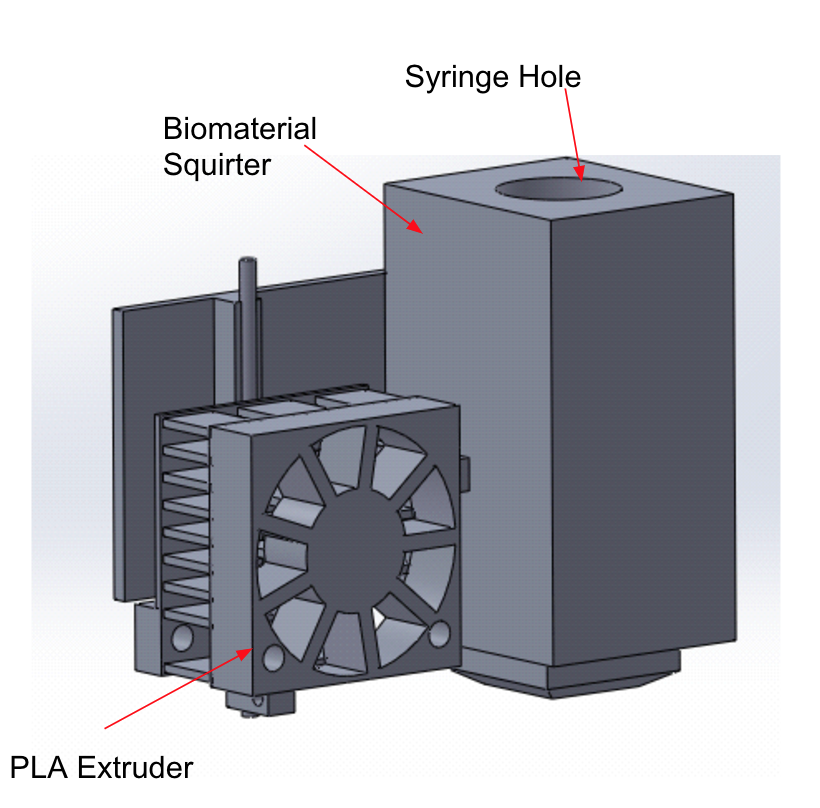
\includegraphics[scale=0.5]{extruder}
\caption{\label{figure:extruder} Rendering of additional PLA extruder module}
\end{figure}

By having a second extruder, the printer can print with both biomaterial and PLA plastic. The module in Figure \ref{figure:extruder} demonstrates how the PLA extruder will be positioned next to the biological extruder. This allows for quick transitions between print materials. 

\begin{figure}[H]
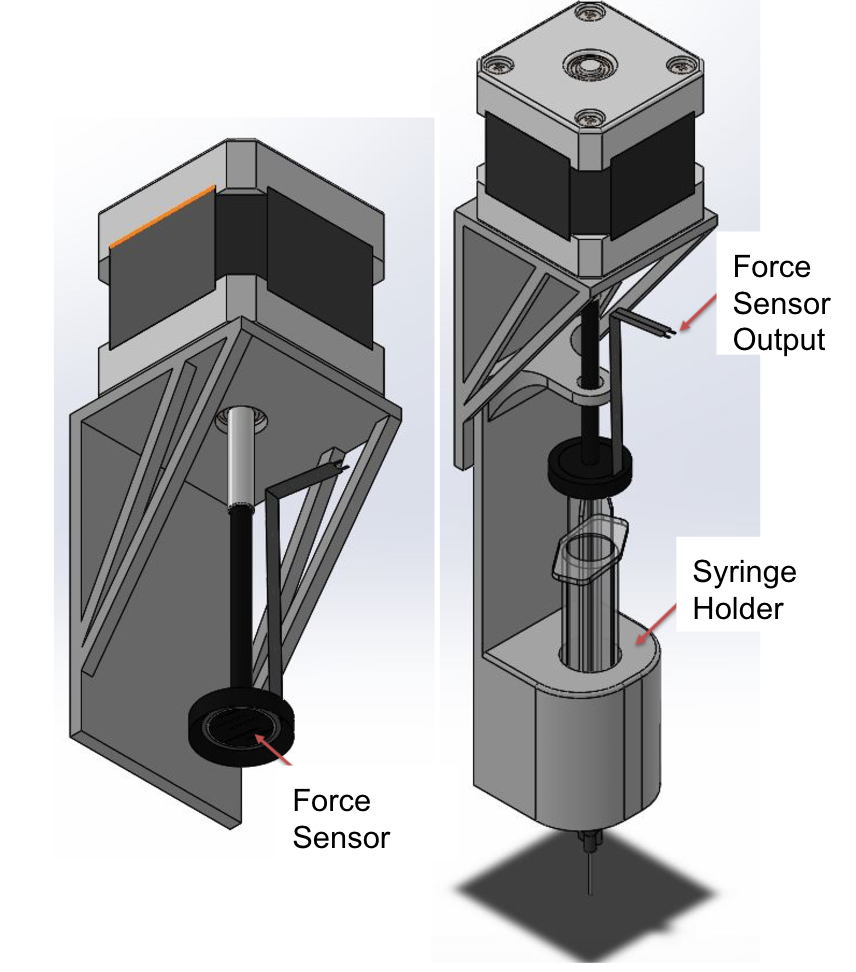
\includegraphics[scale=0.5]{plunger}
\caption{\label{figure:plunger} Rendering of auto-calibration plunger}
\end{figure}

By using a force sensor as shown in Figure \ref{figure:plunger} will be able to detect the amount of force required to drive the plunger. Through testing, we can observe the change in force between various biomaterials and air. Then, we can use the servo motor to drive the plunger until it has been sensed that all of the air has been expelled. 

\section{Technologies Used}
\begin{itemize}
\item Git: A commonly used version control system. Git allows distributed workflow with high data integrity.
\item Arduino Microprocessor: A small, widely used open-source microprocessor commonly used for electronic projects. Arduinos have many controllable input and output pins used to interact with other devices.
\end{itemize}

\section{Design Rationale}

\subsection{Justification for PLA Extruder}
	One of the main features missing from the SE3D printer when compared to other printers in the market is the ability to print with additional materials. By adding a second extruder, the usability of the printer is increased. With the PLA extruder, structural scaffolding can be printed. By using both PLA and biomaterials, more complex structures can be created.

\subsection{Justification for Auto-calibration of Extruder }
	Users of the SE3D printer have given feedback that one of the most difficult aspects for students is proper calibration of the printer. Without proper calibration, prints may fail. By adding auto-calibration to the extruder, we can improve the user experience and decrease the number of failed prints.

\subsection{Justification of Technologies Used}
\begin{itemize}
\item Git: Git was chosen because of its ability to store nearly any type of electronic materials such as images, source code, and documentation. It is commonly used in industry and is well supported. It allows the developers to work concurrently on various parts of the project which results in much faster completion times. Finally, because it is a version control system we can easily reference old code and track changes.

\item Arduino Microprocessor: The Arduino board is commonly used for 3D printers because of its modularity, cheap price, and well supported community. There are many available open-source printer firmwares available that are designed specifically for the Arduino Platform. The Duet board SE3D uses actually switched to Arduino firmware because of the development community around the Arduino Mega. The Arduino can also easily interface with other technologies, such as media readers and LCD screens. Finally, its processor allows for accurate and fast control of stepper motors, which is required for the success of 3D prints.

\end{itemize}

\chapter{Testing Plan}
\chapter{Societal Issues}

\section{Ethical}


\section{Social}


\section{Political}


\section{Health and Safety}
\section{Economic}


\section{Manufacturability}
\section{Sustainability}
\section{Environmental Impact}
\section{Usability}
\section{Lifelong Learning}
\section{Compassion}
\chapter{Conclusion}



\chapter{References}

\begin{hangparas}{1cm}{1}
``Aether Enters 3D Bioprinting Collaboration with Center for Cancer Nano." PRWeb. 2016. Web. 07 Nov. 2016.

``Applications for 3D Printing." EnvisionTEC.Web. 07 Nov 2016.
Bio-3D.com. 

``Bio3D Technologies – Printing and Shaping the Future. "Bio3D Technologies – Printing and Shaping the Future. Web. 07 Nov. 2016.

``Bioprinting of Human Tissues and Organs." Cellink. Web. 07 Nov. 2016.

Gao, Qing et al. “Coaxial Nozzle-Assisted 3D Bioprinting with Built-in Microchannels for Nutrients Delivery.” Biomaterials, vol. 61, 2015, pp. 203–215

Lomas, Natasha. ``BioBots Is A 3D Printer For Living Cells." TechCrunch. 2015. Web. 07 Nov.2016. 

Ozbolat, Ibrahim T., Howard Chen, and Yin Yu. \"Development of ‘Multi-arm Bioprinter’ for hybrid biofabrication of tissue engineering constructs.\" Robotics and Computer-Integrated Manufacturing 30.3 (2014): 295-304.

Rankin, Kyle. \"What's New In 3D Printing, Part IV: OctoPrint.\" Linux Journal 257 (2015): 38-42. Applied Science and Technology Source. Web. 7 Oct. 2016.

``RegenHU | Bioprinting, 3D Bio-printers, Biomaterials – RegenHU." RegenHU | Bioprinting, 3D Bioprinters, Biomaterials – RegenHU. Web. 07 Nov. 2016.

Yordanova, Snejana1. \"Intelligent Approaches For Linear Controllers Tuning With Application To Temperature Control.\" Journal Of Intelligent and Fuzzy Systems 27.6 (2014): 2809-2820. Applied Science and Technology Source. Web. 7 Oct. 2016.

\end{hangparas}
\chapter{Appendices}


\backmatter
\end{document}
